% ============================================================
% Amazon-VT CFP 2026-2027 — 1-Page Abstract v4c
% AKG-E: Construction-Only Variant with VVUQ Backbone
% Primary: AI Accelerated Science & Engineering
% Secondary: Agentic AI
% Format: IEEE 2-column
% ============================================================

\documentclass[conference, 10pt]{IEEEtran}

\usepackage[utf8]{inputenc}
\usepackage[T1]{fontenc}
\usepackage{graphicx}
\usepackage{hyperref}
\usepackage{microtype}
\usepackage{cite}
\usepackage{enumitem}
\setlist{nosep, leftmargin=1.5em, topsep=0.2em}
\usepackage{tikz}
\usetikzlibrary{positioning, arrows.meta, shapes.geometric, fit, calc}

\title{Agentic Knowledge Graphs with Simulation-in-the-Loop Validation\\for Construction Engineering}
\author{}
\date{}

% ============================================================
\begin{document}

\maketitle
\thispagestyle{empty}

\vspace{-1.5em}

\noindent\textbf{Primary Topic:} AI Accelerated Science \& Engineering \hfill
\textbf{Secondary Topic:} Agentic AI

\vspace{0.5em}

AI-driven breakthroughs---from biomolecular structure prediction~\cite{Abramson2024AlphaFold3} to materials discovery~\cite{Merchant2023GNoME}---show that domain-specific AI dramatically accelerates discovery when tightly coupled to structured knowledge and simulation. Construction engineering faces an analogous opportunity: large language models (LLMs) hallucinate physical quantities~\cite{Ji2023HallucinationSurvey}, cannot enforce constraint satisfaction, and lack grounding in the structured ontologies and simulation feedback loops that define engineering workflows. Physics-informed machine learning~\cite{Karniadakis2021PINN} has matured in isolation from generative AI, creating an integration gap between simulation-based engineering and the emerging agentic paradigm.

This project proposes \textbf{Agentic Knowledge Graph Engineering (AKG-E)}, a framework enabling LLM-powered agents to reason over structured construction knowledge, interact with physics-based simulations, and validate outputs through \textbf{Verification, Validation, and Uncertainty Quantification (VVUQ)}~\cite{Oberkampf2010VVUQ}. While VVUQ is well-established for computational simulation, no methodology exists for systematically validating AI agent-generated engineering outputs---a critical trust gap blocking deployment. AKG-E closes this through three layers: (1)~a \textit{domain ontology layer} encoding construction knowledge graphs (KGs) with entities, constraints, building codes, and Building Information Modeling/Industry Foundation Classes (BIM/IFC)~\cite{Eastman2011BIM} design rules; (2)~a \textit{simulation integration layer} exposing finite element analysis (FEA) solvers~\cite{Logg2012FEniCS} as agent-callable interfaces; and (3)~a \textit{VVUQ validation layer} that verifies agent-generated designs against physical laws, quantifies prediction uncertainty via Monte Carlo propagation through agent pipelines, and enforces regulatory constraints. Agents orchestrate across retrieval-augmented generation~\cite{Lewis2020RAG}, structured graph queries~\cite{Edge2024GraphRAG}, and simulation calls.

\begin{figure}[t]
    \centering
    \resizebox{\columnwidth}{!}{%
    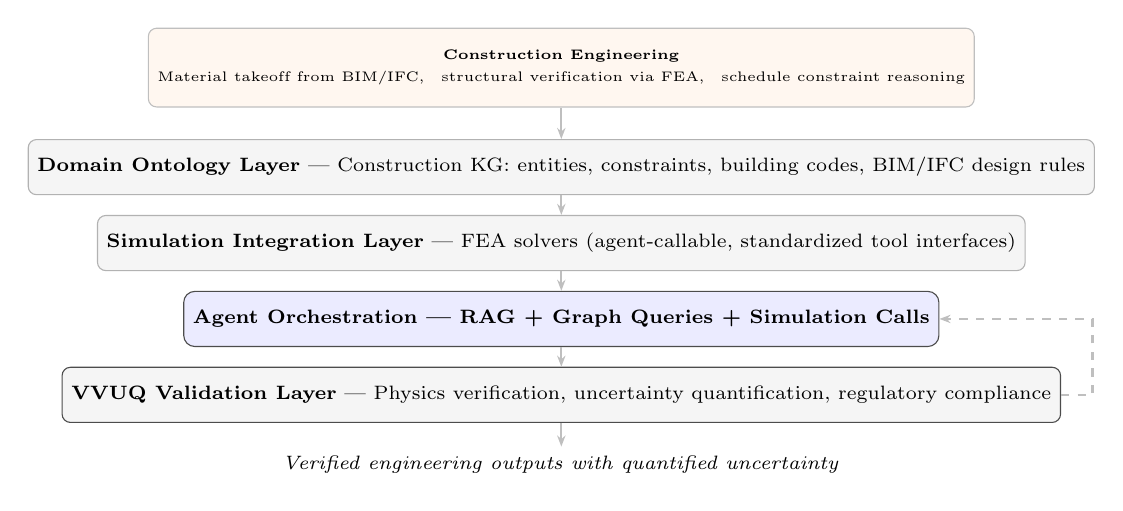
\begin{tikzpicture}[
        node distance=0.35cm and 0.25cm,
        layerbox/.style={rectangle, rounded corners=3pt, draw=gray!60, fill=gray!8, minimum width=7.5cm, minimum height=0.7cm, align=center, font=\scriptsize},
        dombox/.style={rectangle, rounded corners=3pt, draw=gray!50, fill=orange!6, minimum width=7.5cm, minimum height=1.0cm, align=center, font=\tiny},
        agentbox/.style={rectangle, rounded corners=4pt, draw=black!70, fill=blue!8, minimum width=7.5cm, minimum height=0.7cm, align=center, font=\scriptsize\bfseries},
        arr/.style={-{Stealth[length=4pt]}, thick, gray!50},
    ]
        % Domain application (top) - single construction domain
        \node[dombox] (con) {\textbf{Construction Engineering}\\[2pt]\tiny Material takeoff from BIM/IFC,\;\; structural verification via FEA,\;\; schedule constraint reasoning};

        % Domain ontology layer
        \node[layerbox, below=0.4cm of con] (onto) {\textbf{Domain Ontology Layer} --- Construction KG: entities, constraints, building codes, BIM/IFC design rules};

        % Simulation integration layer
        \node[layerbox, below=0.25cm of onto] (sim) {\textbf{Simulation Integration Layer} --- FEA solvers (agent-callable, standardized tool interfaces)};

        % Agent orchestration
        \node[agentbox, below=0.25cm of sim] (agent) {Agent Orchestration --- RAG + Graph Queries + Simulation Calls};

        % VVUQ validation
        \node[layerbox, below=0.25cm of agent, draw=black!70] (val) {\textbf{VVUQ Validation Layer} --- Physics verification, uncertainty quantification, regulatory compliance};

        % Output
        \node[font=\scriptsize, below=0.3cm of val] (out) {\textit{Verified engineering outputs with quantified uncertainty}};

        % Arrows
        \draw[arr] (con) -- (onto);
        \draw[arr] (onto) -- (sim);
        \draw[arr] (sim) -- (agent);
        \draw[arr] (agent) -- (val);
        \draw[arr] (val) -- (out);

        % Feedback loop
        \draw[arr, dashed] (val.east) -- ++(0.4,0) |- (agent.east);
    \end{tikzpicture}
    }%
    \caption{\textbf{AKG-E Framework (Construction).} The construction domain plugs into shared ontology, simulation, and VVUQ layers. Agents orchestrate retrieval, graph reasoning, and FEA calls; the VVUQ layer verifies outputs, quantifies uncertainty, and enforces building codes, with a feedback loop for iterative refinement.}
    \label{fig:framework}
    \vspace{-0.5em}
\end{figure}

In \textbf{construction engineering}, agents parse BIM/IFC~\cite{Eastman2011BIM} models to extract structural elements and populate a construction KG encoding materials, loads, and code requirements. Three core tasks drive the evaluation: (i)~\textit{material takeoff}---automated extraction of bill-of-materials from IFC files, validated against code-compliant quantities; (ii)~\textit{structural verification}---FEA~\cite{Logg2012FEniCS} calls for load analysis, with VVUQ ensuring safety margins and quantifying material-property uncertainty via Monte Carlo propagation; and (iii)~\textit{schedule constraint reasoning}---agents flag sequencing conflicts before construction begins, with constraint violations logged for human review. The framework targets deployment on Amazon Bedrock~\cite{AWSBedrockHybridSearch2024}, enabling integration with existing AWS data pipelines and document repositories without specialized on-premises infrastructure.

We test one falsifiable hypothesis: \textbf{VVUQ-gated agents will reduce constraint violation rates versus unconstrained LLM baselines by measurable margins} on construction benchmarks (target: $>$50\% reduction). A secondary hypothesis holds that VVUQ-aware pipelines yield calibrated uncertainty estimates for structural quantities (coverage within 10\% of nominal), enabling principled thresholds for autonomous versus human-reviewed decisions.

Experiments compare prompt-only LLMs, RAG-augmented baselines~\cite{Lewis2020RAG}, and full AKG-E across all three task types using expert-annotated ground truth from BIM models. Deliverables include the open AKG-E framework, VVUQ-integrated KG templates for BIM/IFC workflows, and benchmarks demonstrating that \textbf{simulation-grounded agentic AI} outperforms unstructured approaches for construction decision-support.

\bibliographystyle{IEEEtran}
\bibliography{references}

\end{document}
